\section{Implementering af tilpasning af træningsniveau}
I tilpasningcontrolleren beregnes den andbefalede træningstid. Dette gøre ud fra kategorisering, den daglige helbredstilstand og en tidligere evaluering, fortaget efter samme træningsform, -type og heldbredstilstand.
Beregningen for den anbefalede træning er implementeret ved brug af if/else statement. Et udpluk af denne beregning fremgår af \autoref{fig:anbekode}.  
   
\begin{figure} [H]
\centering
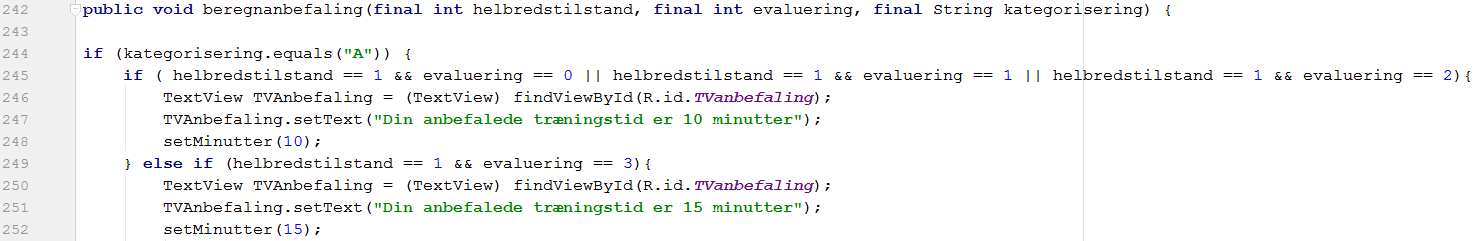
\includegraphics[width=1\textwidth]{figures/imple/anbekode}
\caption{Udpluk af koden for anbefalet træning. If/else løkker afgør, hvilket træningsniveau brugeren får anbefalet.}
\label{fig:anbekode}
\end{figure} 

\noindent
Af figuren ses beregningen af den anbefalede træningstid for brugeren med kategorisering "A" og heldbredstilstanden på "2". Variationen for anbefalingen afhænger af evalueringen og kan i dette eksempel variere mellem "15", "20" og "25 minutter". Metodekaldet \textit{setMinutter} referer til, at der sættes en bemærkning idet den anbefaldede træningstid er opnået.
